\chapter{Object detection}
Object detection is another prevalent task in the domain of computer vision.
An object detection task is one where the goal is to localize one or many different classes of objects using bounding boxes.
Before current deep learning-based techniques, a popular way to solve the problem was to use handcrafted features like in image classification and to use a sliding window over the image for localizing objects.
These previous techniques include, for example, the Viola-Jones detector \citep{viola-jones}, which uses a sliding window and AdaBoost for features, and another popular method was using histograms of oriented gradients \citep{hogs} to find where the boundaries of objects exist.
These days there exist various ways of using the feature maps of neural networks for learning the filters to get much better results.
The various architectures can be split into two approaches, one-stage detectors, and two-stage detectors.
The two-stage detectors require region proposals, based on which the object detection is done.
An often-used family of these kinds of methods is the R-CNN classifiers, for example, the faster R-CNN \citep{faster-rcnn}.
In the one-stage detectors, features from various layers of the classifier are used to get the predictions.
For example, the YOLOv4 \citep{yolov4} is the 4th iteration of the single-stage YOLO family of detectors that are very popular due to the good balance between fast speed and good accuracy.

\begin{figure}[h!]
    \centering
    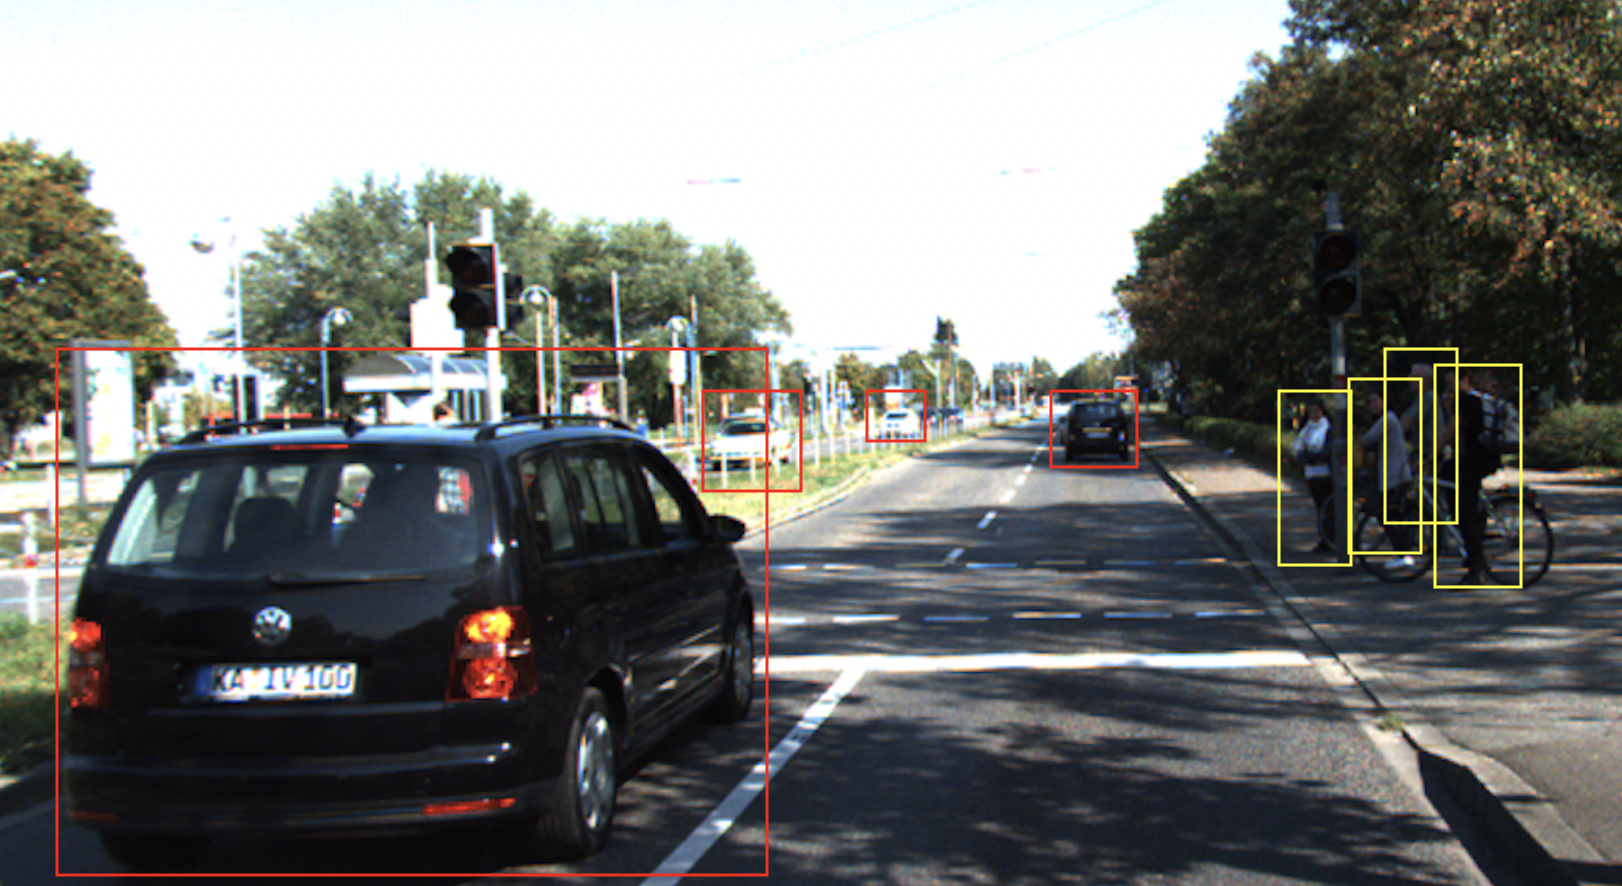
\includegraphics[width=0.8\textwidth]{imgs/obj-det.png}
    \caption{Object detection image labeled for people and cars.}
\end{figure}

\section{Metrics}
The training of object detection models requires data sets that have been labeled for that purpose.
Generally, the data sets contain bounding box annotations for each of the classes in the data set, such as seen in Figure 5.1.
For this reason, object detection models can't use a simple metric like the basic accuracy in image classification.
As the images are often manually labeled, the boxes are most likely not completely consistent.
So most likely, the predictions are never going to align with the labeled boxes perfectly.
Consequently, the method for evaluating object detection performance is Average Precision (AP) or mean Average Precision (mAP) or one of their variants.
These metrics use intersection over union (IoU) score to evaluate how incorrect the predicted bounding box is when compared to the actual label. Intersection over union is visualized in Figure 5.2.

\begin{figure}[h!]
    \centering
    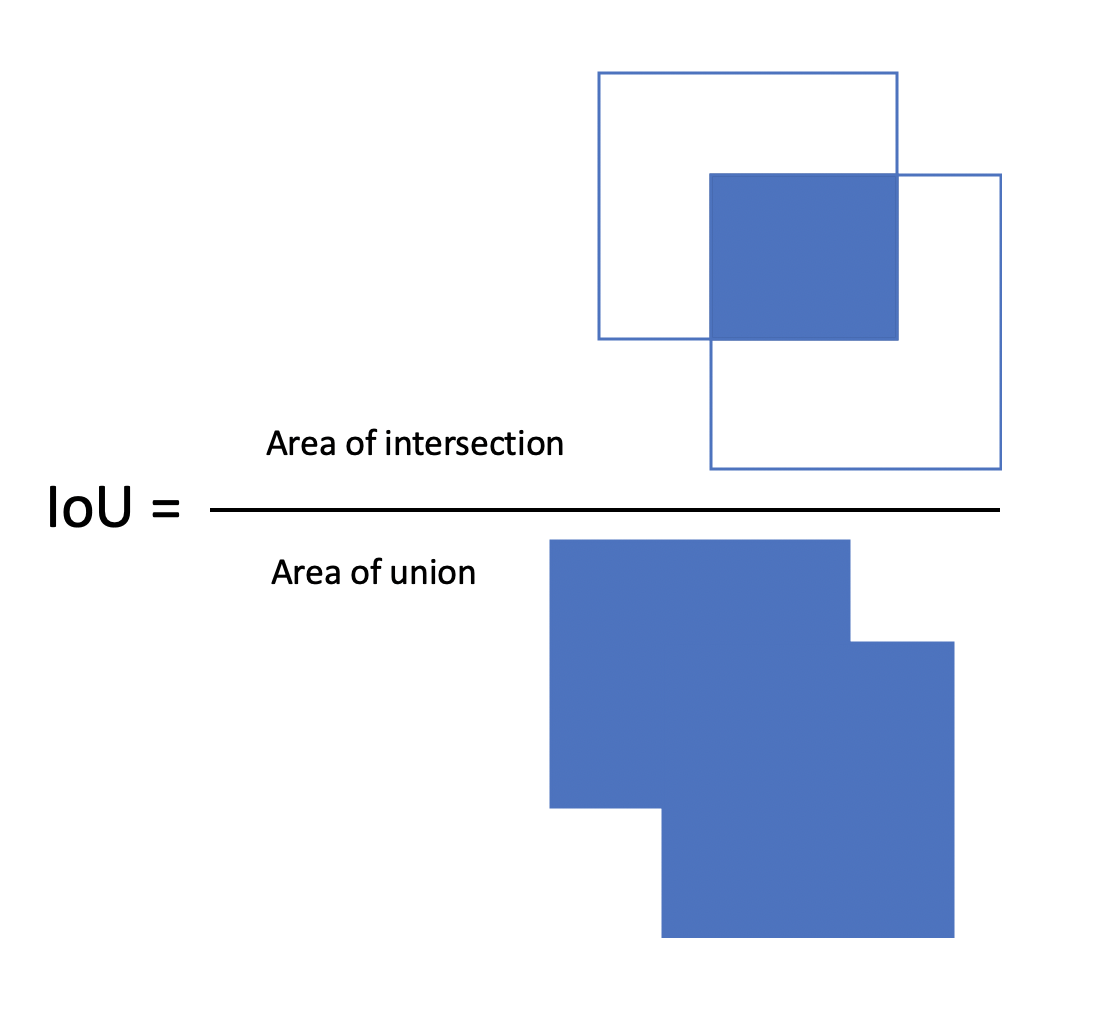
\includegraphics[width=0.8\textwidth]{imgs/IoU-own.png}
    \caption{The visual formula for calculating intersection over union.}
\end{figure}

To get to a final AP score, the first thing that has to be decided is the IoU score threshold for considering a prediction to be correct.
For example, we could consider all predictions that have over 50\% or 75\% overlap in the IoU.
The threshold value for IoU that should be used is not entirely standardized, and there are multiple ways of calculating the AP score.
For example, the popular COCO dataset \citep{COCO} uses an average of 10 IoU scores ranging from .5 to .95 IoU thresholds as the main metric.
To get the AP for a class, we need to graph the precision-recall curve and then calculate the area under it.
For example, the Pascal Visual Object Classes Challenge (VOC) \citep{PVOC} recommends doing this by using 11 points of interpolated precision.
So we get the following formula for Average Precision:

\[AP = \frac{1} {11} \sum_{r \in \{0, 0.1, \ldots, 0.9 , 1\}}{p_{interp}(r)}\] \noindent

Where $p_{interp}$ is defined as

\[p_{interp}(r) = \max \limits_{\tilde{r}:\tilde{r} \geq r} p(\tilde{r})\]

Then to get the mAP score, we can average the AP score for each of the classes in the data set.
As was mentioned, this way of calculating the AP is not always the same, for example, the COCO metrics \citep{COCO_SITE} recommend using 101 points for integrating the curve instead of the 11 proposed in the VOC.
This discrepancy in the integration means that not all AP scores are directly comparable.

\section{Object detection model structure}
Much like image classifiers and many other vision tasks, modern object detectors rely on pre-trained backbones to generate the features required for predicting bounding boxes.
A classifier head is required to get these predictions, but in object detectors, this head is more complicated than in image classification.

For the backbone, most object detection architectures use one of the same ImageNet models as in image classification such as ResNet or VGG.
However, the YOLO models use DarkNet, which is specifically designed for achieving efficient results in object detection \citep{yolov4}.
The main reason for picking one backbone over another is often a function of both accuracy and inference time.
As object detectors are often run on video data, inference time can be more significant than in image classification, as it is often desirable to be able to run them in real-time.

The head is where the architectures differ the most, and generally, any backbone could be combined with a specific detector head.
The head comprises of a neck, which connects the intermediate features from the backbone to the final head.
The intermediate features are generally connections from some specific layers of the backbone.
Earlier single-stage detectors used the extracted features directly, but the current state-of-the-art methods use special feature pyramids and path aggregation to get the best results \citep{efficientDet}.
For example, the YOLO v4 uses spatial pyramid pooling \citep{SPP} over the DarkNet features and path aggregation net (PANet) \citep{PANET} to concatenate the parameters for the classifier head \citep{yolov4}.
Different ways of combining the feature pyramids are described in Figure 5.3.
Like many other parts of the architecture, picking one is a trade-off of more parameters and inference time and accuracy.
\begin{figure}[h!]
    \centering
    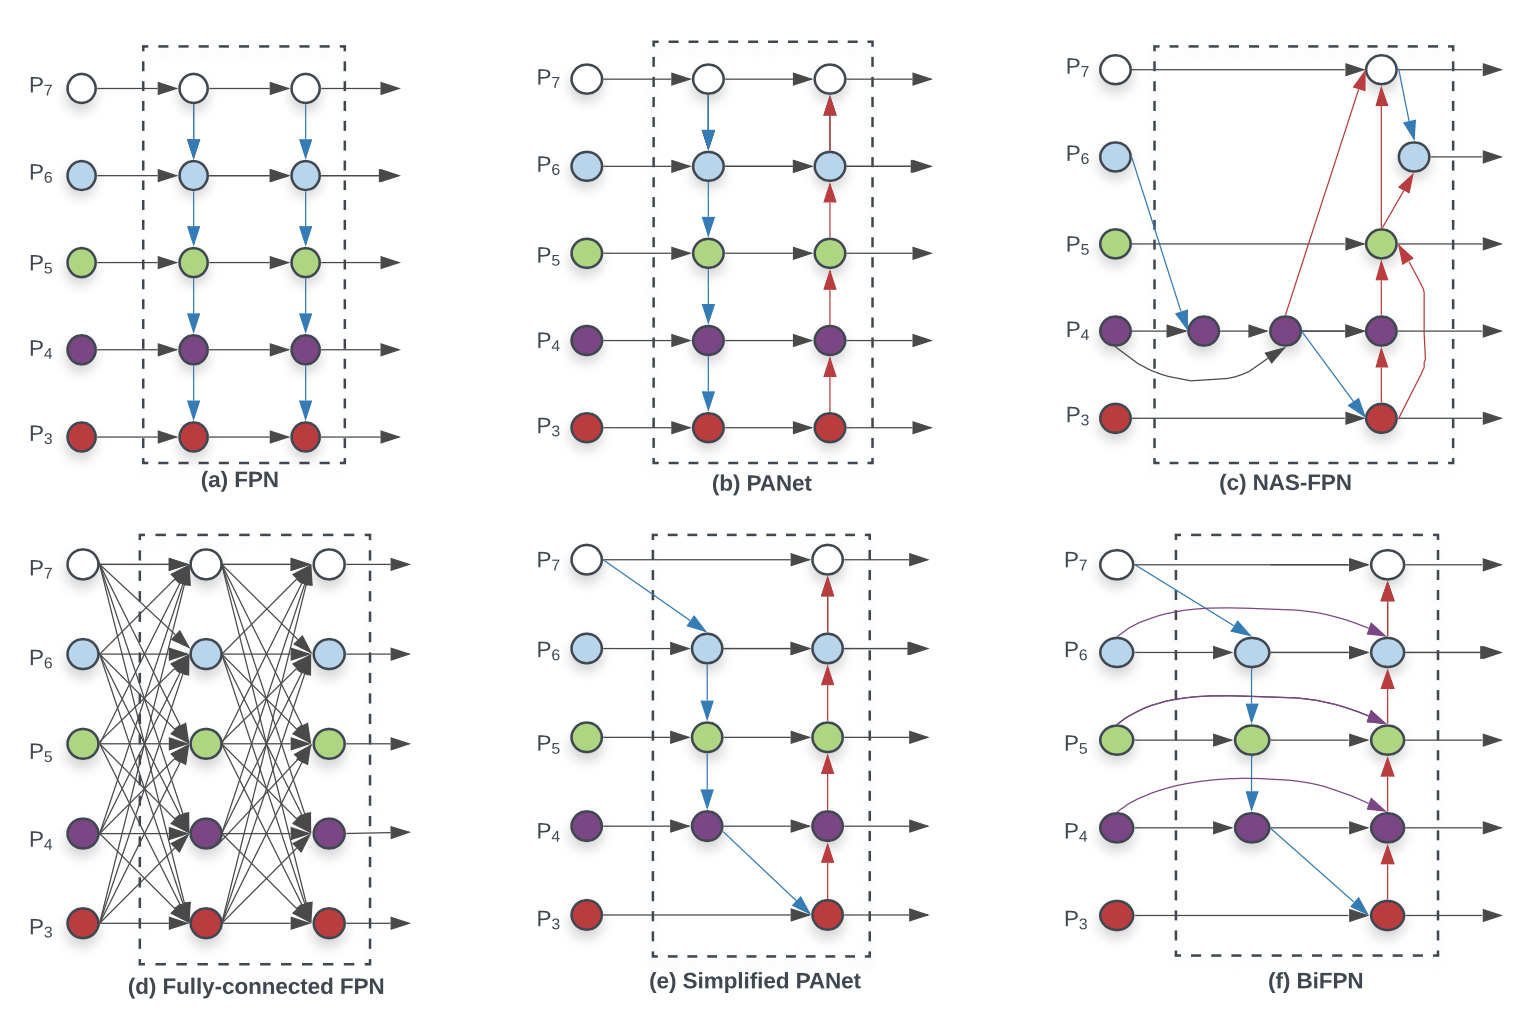
\includegraphics[width=0.8\textwidth]{imgs/detector_necks.png}
    \caption{a) Basic FPN \citep{FPN} where features are combined in only one direction. b) PANet modifies the basic FPN by adding a path from the lower level features to higher-level features. f) BiFPN tries to prune the connections to the most important ones. Image adapted from \citep{efficientDet}.}
\end{figure}

In two-stage detectors like faster R-CNN \citep{faster-rcnn}, there is a region proposal network (RPN), which predicts region proposals using a sliding window for some anchor boxes.
Running this RPN is expensive, and often the two-stage models are much slower than the single-stage detectors.
The benefit of the two-stage approach is generally a better accuracy. 
Still, recently the one-stage methods like YOLO v4 have achieved very similar accuracies to the two-stage ones with much faster inference times \citep{yolov4}.
By utilizing new ways of using the feature maps, the object detectors have recently become significantly better over the years, as can be seen from the different iterations of the YOLO models, as they have been using very similar backbones over the years \citep{yolov4}.

\section{Multi-dataset training}
Often an object detection problem requires detecting multiple different classes in a similar context.
For example, a self-driving car would need to detect various traffic signs, cars, pedestrians, road markings, cyclists, and many other things.
Collecting a single dataset that has labels for all of the classes of interest can be a very daunting task.
Even if it is feasible to create the dataset for the original classes of interest, this approach does not scale very well when new classes need to be recognized.
As likely the original dataset might contain millions of images labeled for multiple classes, adding a new class would require going through the entire dataset again and labeling the new class as well.
The new class may be relatively rare; for example, we may be interested in detecting emergency vehicles with sirens on.
Here is where multi-dataset learning is highly beneficial as it only allows for collecting a specific class dataset.
This type of cross-dataset learning is useful when we need to combine multiple distinct data sources to detect some union of the labels \citep{cross_data}.

The main difficulty in combining multiple datasets for detection lies in the fact that they likely contain unlabeled overlapping classes.
For example, given a dataset for detecting cars and another for detecting stop signs, we have two distinct datasets where only one of the classes is labeled.
If we train this model, assuming that the labels are genuinely valid, we will end up unlearning the tasks due to the overlap of the classes.
The problem lies in the fact that it is most likely that in the car dataset, we will find stop signs that are not labeled.
Similarily we will find cars that are unlabeled within the stop sign dataset.
When we naively train this model, we will end up detecting cars and stop signs that are actually correct but incorrect based on the labels.
The model will be punished for detecting these non-labeled positive examples due to the absence of the labels.

One way to do this is by disallowing the labels from incorrect datasets affecting the total loss.
For example, in \citep{cross_data}, the RetinaNet \citep{retinaNet} model's loss function is modified to ignore the losses for tasks that are not a part of the dataset.
All models using the same focal loss as RetinaNet can be trained with this adjusted loss function.
This way, each class will get its own positive and negative dataset to train on and not affect the performance of the other classes.
Still, this does not completely solve the problem as some of the classes might require conflicting features, as can be the case when very different tasks are combined. 
In that case, it could be smart to split the similar classes into different detectors and maybe share only the lower levels between all tasks.

Similar multi-dataset training can also be applied in multi-label image classification settings.
A multi-label image classification problem is one where we want to assign multiple labels to an image.
For example, we might want to classify whether it is raining, the sun is shining, the sea is visible, is there a dog in the image, and so on for all the classes of interest.
Again, collecting a dataset containing all labels for all images is quite expensive, but we can train this with a separate binary classification head for each task.
And as collecting a separate dataset for each task is relatively easy, it is possible to create a quite powerful model with relative ease.

\section{EfficientDet}
EfficientDet \citep{efficientDet} is an object detection model, that is based on the previously covered EfficientNet ImageNet model.
The neck for the EfficientDet is a unique bidirectional feature pyramid network (BiFPN).
The EfficientDet model also uses similar compound scaling as the EfficientNet models for the new object detection specific parts.
The scaling factor is used for the BiFPN network, box and class predictor networks, and to find the optimal input resolution.
The EfficinetDet shows that improving the backbone is quite useful for the entirety of the model.
This can especially be seen when looking at the comparisons of using a ResNet vs an EfficientNet as the backbone in the same EfficientDet architecture \citep{efficientDet}.
The EfficientDet model architecture is shown in Figure 5.4.

\begin{figure}[h!]
    \centering
    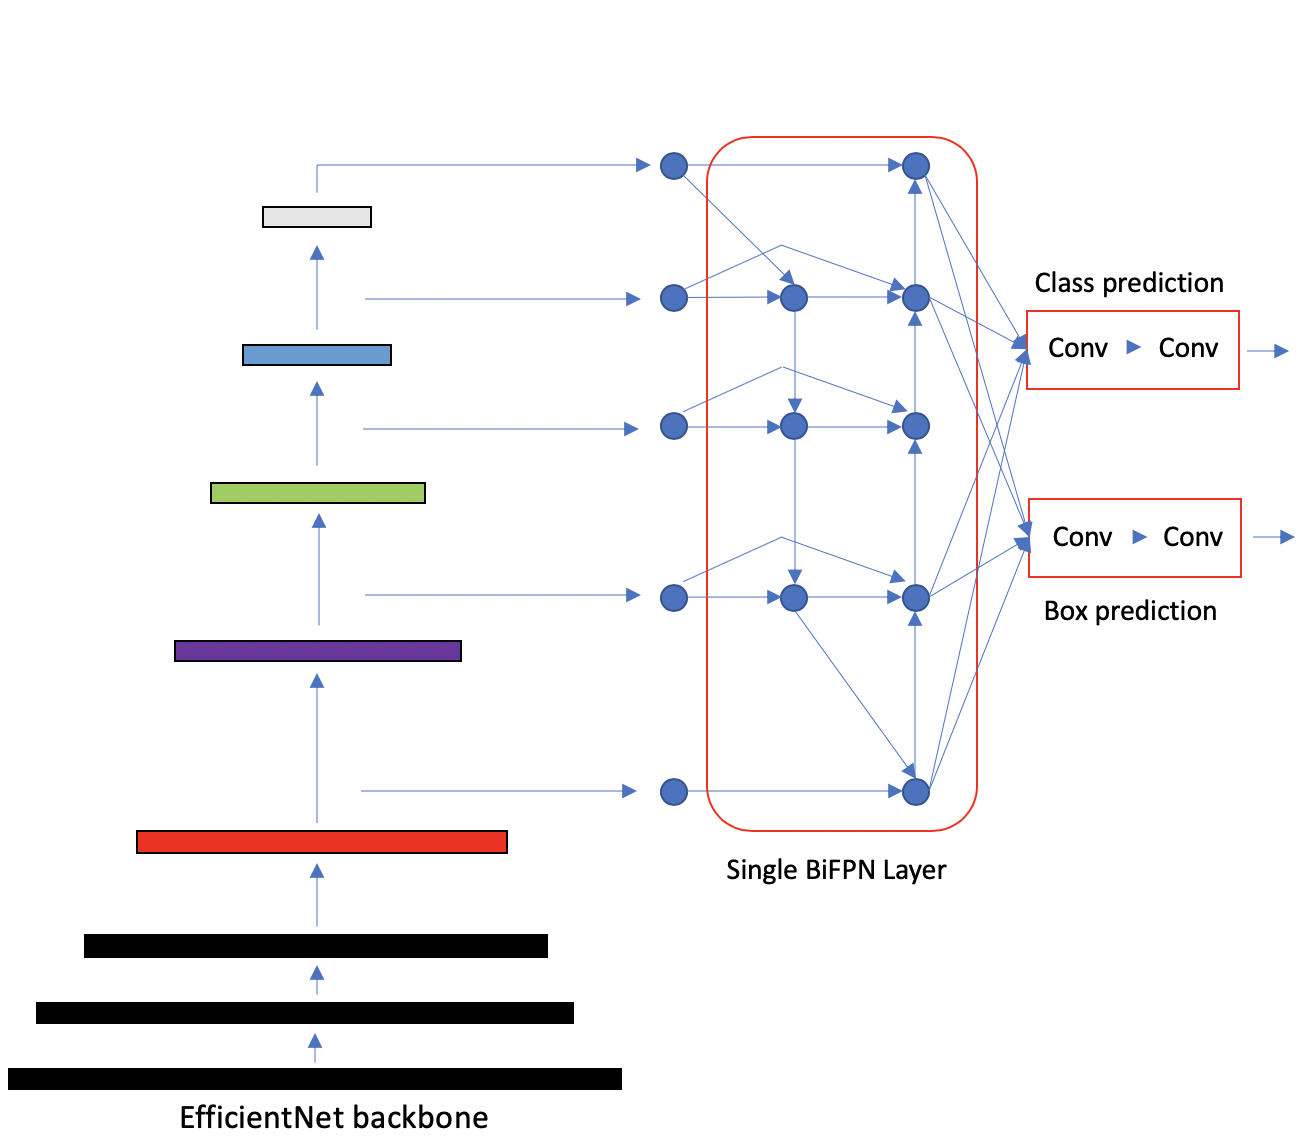
\includegraphics[width=0.8\textwidth]{imgs/eDet-own.png}
    \caption{EfficientDet architecture comprises of the EfficientNet \citep{efficientNet} backbone, the bidirectional feature pyramid network neck and the class and box classifier heads. Here only one BiFPN layer is pictured, but there are multiple of them normally stacked in succession.}
\end{figure}

The different feature maps in the BiFPN are combined using a weighted feature fusion.
The feature maps can't be directly combined since they have different dimensionality, so they have to be up or downsampled depending on the direction of the connection.
By weighing each feature map, the network can learn how important each feature map is.
Since the dimensionalities differ from one another, they likely don't contribute equally to the output feature maps, which is signified by the learned weight.
The BiFPN connection architecture is a simplified version of the PANet, as shown in Figure 5.3.
The goal of the changes from PANet is to have a more high-level fusion of features while dropping the nodes that have little feature fusion and then to stack multiple of these layers to get the final model \citep{efficientDet}.

The efficient scaling of the parameters and the BiFPN architecture allow EfficientDet to produce impressive results at relatively high framerates.
The new YOLO v4 produces very similar scores at acceptable framerates also \citep{yolov4}.
Still, some slightly better results are produced by the two-stage detectors, but those can't reach a 30 FPS inference time \citep{yolov4}.
So in practice, using either the EfficientNet or YOLO is a good idea when video needs to be classified.
The EfficientNet scales relatively well with larger EfficientNet backbones, but it is not possible to classify real-time video.
This flexibility allows for picking the model with a suitable accuracy for the problem at hand.

\section{Training object detectors}
As we described previously, object detectors are trained when there is a need to localize some set of classes within images by describing them with bounding boxes.
One widely used format for labeling such a dataset is the format for the object detection data in the COCO data set.
The COCO data consists of a set of images and a separate JSON file containing the labels.
The label file contains a list of all the images for the data set and a unique identifier for each image.
There is also an annotation list that contains a list of objects that specify the bounding box annotations.
The annotations are specified as being linked to a single image by its image id and defining the bounding box annotation dimensions.
The bounding box annotations are formatted by providing the coordinates of the top-left corner of the annotations and then the width and height of the box, so it is a tuple of four numbers (x, y, width, height).
To train on new data sets, they should be formatted similarly to make the training as easy as possible.

Once the data set has been gathered and collected in a correct format for the object detection task, a model needs to be picked.
Here, the final inference model's requirements need to be evaluated to decide whether a single-stage or a two-stage detector should be used.
For example, when running the model in real-time, a single-stage detector might be better, and in the case of doing text detection, it seems to be more popular to use a two-stage detector.
We will describe here how things work for the EfficientDet, which is a single-stage detector.

Once the exact architecture has been chosen, an implementation of it is needed to construct the model.
Generally, all the popular architectures have open-source implementations on GitHub in both Tensorflow and Pytorch, which are the most popular deep learning frameworks, that can be used.
Most of these implementations come quite readily wrapped in a way that given a correctly formatted data set, the models will be automatically initialized with the correct number of classes, and the training process is already specified by the input of a few necessary parameters.
As mentioned in the case of image classification, it is extremely important to initialize with the pre-trained weights with an object detection model to achieve the best results instead of training from scratch.
In an object detector, the problem-specific part is the number of classes in the classification head, which can be seen in Figure 5.4.
For the rest of the network, pre-trained weights should be used.

Training the EfficientNet itself is a multi-task training problem. 
We have two losses, the regression loss signifying how close the bounding boxes are to the annotations by calculating IoU and classification loss, which tells how incorrect the predicted labels are.
A major problem in optimizing anchor-based single-stage detectors like the EfficientDet is the fact that between the background no-class and the foreground classes of interest, there is a massive discrepancy in the number of instances to classify \citep{retinaNet}.
The anchor-based detectors determine whether an anchor placed at any valid spot in the image contains a class of interest or the background. 
There are tens of thousands to hundreds of thousands of valid anchors to consider depending on the architecture. 
Due to this, we can have a class imbalance of 1:1000 between the positive and negative cases.
For this reason, the recent single-stage detectors use a focal loss presented in the RetinaNet paper, to account for this class imbalance \citep{retinaNet}.

The focal loss introduces two new parameters to the cross-entropy formula to account for the class imbalance. 
The formula for focal loss (FL) is as follows.
\[FL(p_i) = -\alpha_i * log(1-p_i)^\gamma * log(p_i)\] \noindent
Where $\alpha$ and $\gamma$ are the new scaling factors and $p_i$ is defined as $p$ if y = 1 and $1 - p$ otherwise.
The factor $\alpha$ is there to weight the loss for the positive and negative cases separately. 
It is a parameter that is recommended to be set at the inverse class frequency, but the value can be searched by experimentation as well \citep{retinaNet}.
The factor $\gamma$ makes sure that a large number of easy classifications do not dominate the total loss.
For $\gamma$ the recommended value is two \citep{retinaNet}.
With this loss function, it is possible to have a very large number of anchors, where a large majority of them are always predicted as the background class.

With these, the object detection model can be trained.
Still, just leaving all the extra parameters at the default values may not produce the best results.
For example, the possible anchors that the model uses are specified using specific parameters.
The parameters that can be modified are the anchor size, depending on whether large or small objects need to be detected, the anchor sizes can be modified to suit the task at hand.
The anchors also have aspect ratios applied to them, which can be modified, the default ratios are 1:1, 2:1, and 1:2. 

\begin{figure}[h!]
    \centering
    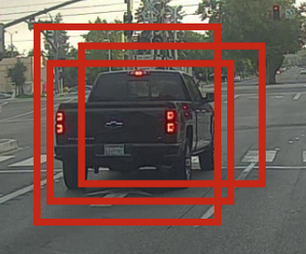
\includegraphics[width=0.8\textwidth]{imgs/nms.png}
    \caption{Object detection without non-max suppression. The same car is detected multiple times.}
\end{figure}

Finally, once a model has been trained with a suitable dataset, architecture, and hyperparameters, it can output predictions for new images.
If the model is used without any modifications, the output boxes will likely look like the predictions in Figure 5.5.
To fix this issue in the predictions, non-max suppression (NMS) should be used \citep{nms}.
With non-max suppression, we can achieve only a single bounding box that better represents what is most likely wanted.
In some cases, using NMS can lead to not being able to predict heavily overlapping classes.
Generally, though NMS should pretty much always be used to avoid the issue depicted in the Figure 5.5.

The object detectors are a good example of multi-task learning and how using the same feature maps, it is possible to solve multiple problems.
In this case, only a single annotation is needed to label for the two different tasks that can be optimized together.
Since we have two losses that are calculated, we can decide to focus on one of the losses by adding a multiplier to it and see if the higher loss could improve that task.
While some of the things covered here will be similar in the two-stage detectors, the region proposal network approach is very different from the anchor-based single-stage detectors covered in this section.
